\documentclass[noinstructornotes]{ximera}
%handout:  for handout version with no solutions or instructor notes
%handout,instructornotes:  for instructor version with just problems and notes, no solutions
%noinstructornotes:  shows only problem and solutions

%% handout
%% space
%% newpage
%% numbers
%% nooutcomes

%I added the commands here so that I would't have to keep looking them up
%\newcommand{\RR}{\mathbb R}
%\renewcommand{\d}{\,d}
%\newcommand{\dd}[2][]{\frac{d #1}{d #2}}
%\renewcommand{\l}{\ell}
%\newcommand{\ddx}{\frac{d}{dx}}
%\everymath{\displaystyle}
%\newcommand{\dfn}{\textbf}
%\newcommand{\eval}[1]{\bigg[ #1 \bigg]}

%\begin{image}
%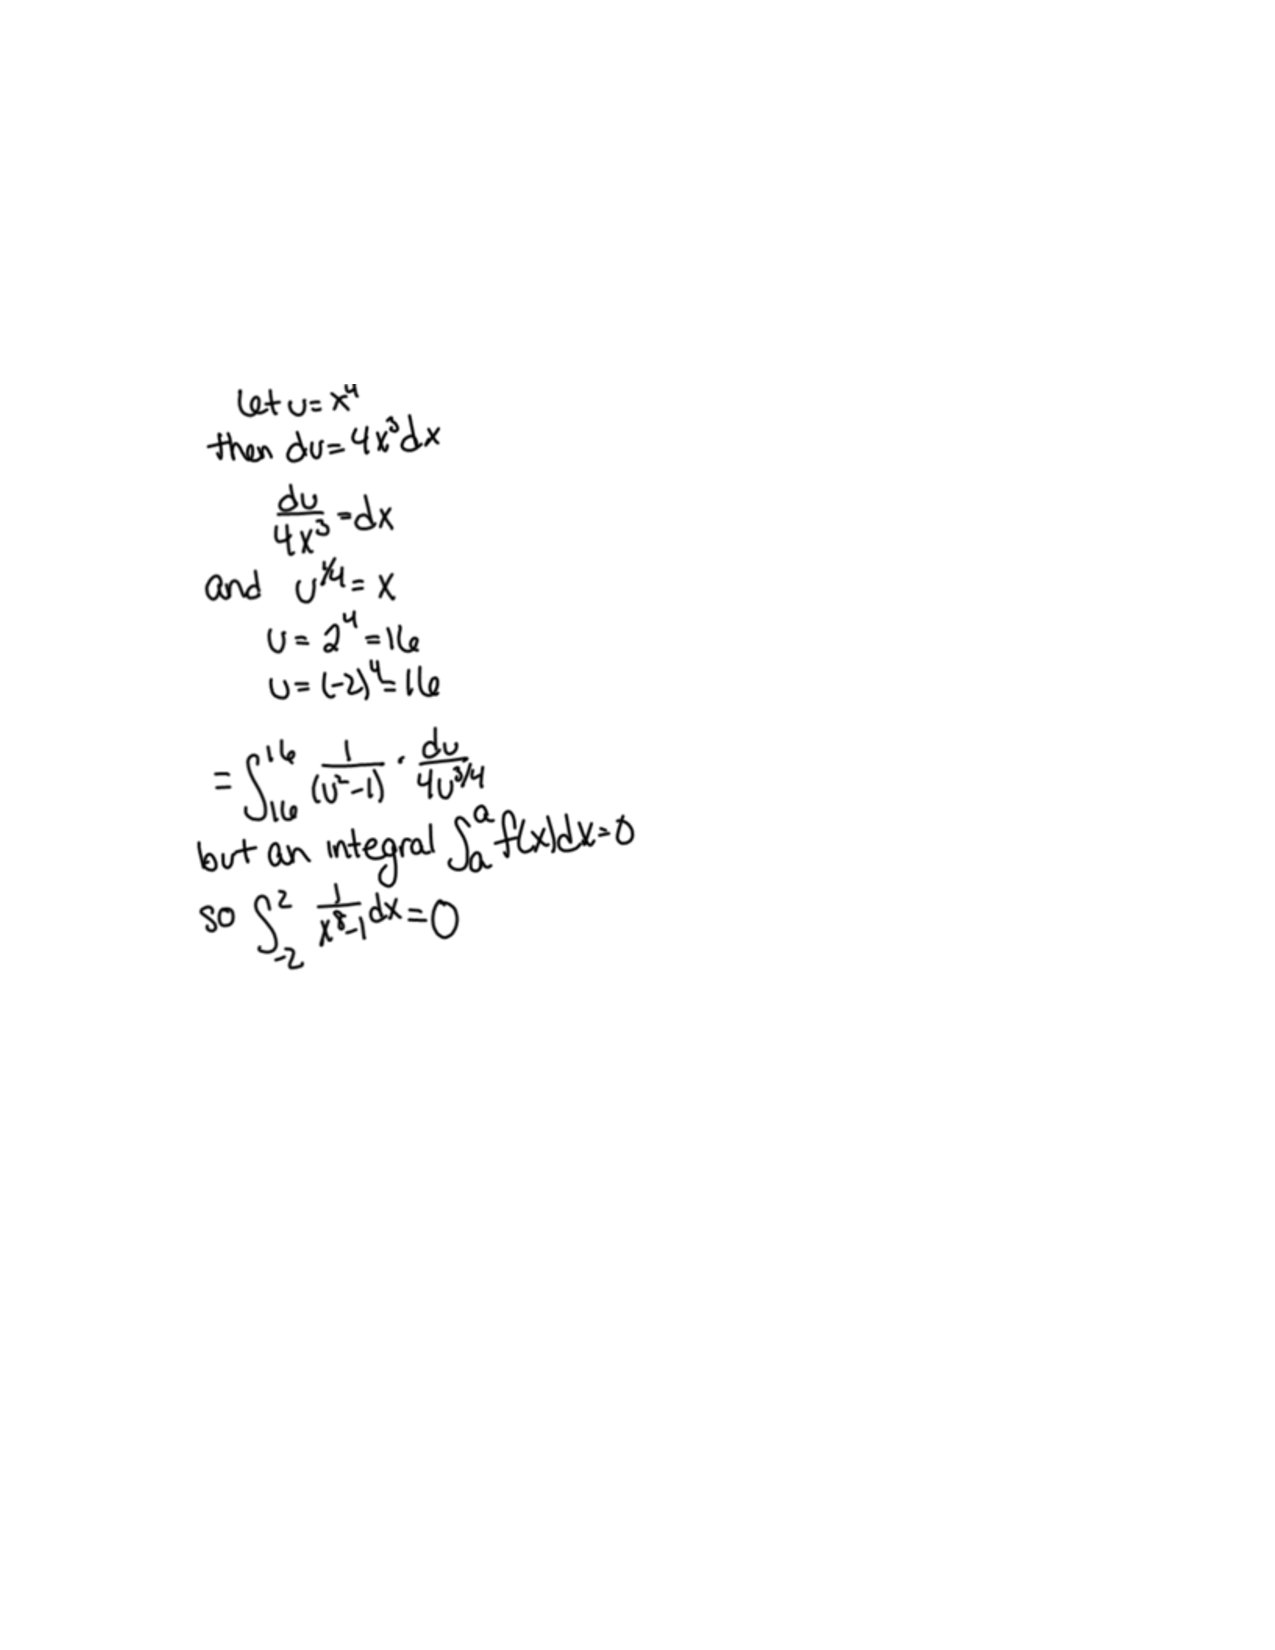
\includegraphics[trim= 170 420 250 180]{Figure1.pdf}
%\end{image}

%add a ``.'' below when used in a specific directory.
\newcommand{\RR}{\mathbb R}
\renewcommand{\d}{\,d}
\newcommand{\dd}[2][]{\frac{d #1}{d #2}}
\renewcommand{\l}{\ell}
\newcommand{\ddx}{\frac{d}{dx}}
\newcommand{\dfn}{\textbf}
\newcommand{\eval}[1]{\bigg[ #1 \bigg]}

\usepackage{multicol}

\renewenvironment{freeResponse}{
\ifhandout\setbox0\vbox\bgroup\else
\begin{trivlist}\item[\hskip \labelsep\bfseries Solution:\hspace{2ex}]
\fi}
{\ifhandout\egroup\else
\end{trivlist}
\fi} %% we can turn off input when making a master document

%\usepackage{fullpage}

\title{Section 8.1: Basic Ideas of Differential Equations}  

\begin{document}
\begin{abstract}		\end{abstract}
\maketitle


\begin{comment}

\section{Warm up:}

\begin{problem}
	
\begin{instructorNotes}

\end{instructorNotes}
\end{problem}

\end{comment}



\section{Group work:}


%problem 1
\begin{problem}
Which of the following is a solution to the differential equation $$y'' + 9y = 0?$$
	\begin{enumerate}
	\item  $y=e^{3t}+e^{-3t}$
	\item  $y=C(t^2 + t)$
	\item  $y=\sin(3t) + 6$
	\item  $y=5 \cos(3t) - 7 \sin(3t)$
	\item  $y=A \cos(3t) + B \sin(3t)$ \text{ (where A and B are real numbers.)}
	\end{enumerate}
	
	\begin{freeResponse}
	\begin{enumerate}
	
	\item  \[ y = e^{3t}+e^{-3t} 	\qquad	y'=3e^{3t}-3e^{-3t} 	\qquad	y''=9e^{3t}+9e^{-3t} \]  
	So,
		\begin{align*}
		y''+9y &= (9e^{3t}+9e^{-3t}) + 9\cdot (e^{3t}+e^{-3t})  \\
		&= 18e^{3t} + 18e^{-3t} \neq 0.
		\end{align*}
	Therefore, this is \dfn{not} a solution to $y''+9y=0$.
	
	
	
	\item  \[ y = C(t^2+t) 	\qquad	y'=C(2t+1) 	\qquad	y''=2C \] 
	So,
		\begin{align*}
		y''+9y &= 2C + 9C(t^2+t)  \\
		&= 9Ct^2 + 9Ct + 2C \neq 0 \text{ if } C \neq 0.
		\end{align*}
	Therefore, this is \dfn{not} a solution to $y''+9y=0$ unless $C=0$, in which case we get the {\it trivial} solution.
	
	
	
	\item  \[ y = \sin(3t)+6 	\qquad	y'=3\cos(3t) 	\qquad	y''=-9\sin(3t) \]  
	So,
		\begin{align*}
		y''+9y 
		&= -9\sin(3t) +9(\sin(3t) + 6)  \\
		&= 54 \neq 0.
		\end{align*}
	Therefore, this is \dfn{not} a solution to $y''+9y=0$.
	
	
	
	\item  \[ y = 5\cos(3t)-7\sin(3t) 	\qquad	y'=-15\sin(3t)-21\cos(3t) 	\qquad	y''=-45\cos(3t)+63\sin(3t) \]  
	So,
		\begin{align*}
		y''+9y 
		&= -45\cos(3t)+63\sin(3t) +9(5\cos(3t)-7\sin(3t))  \\
		&= -45\cos(3t)+63\sin(3t) + 45\cos(3t) - 63\sin(3t) = 0.
		\end{align*}
	Therefore, this \dfn{is} a solution to $y''+9y=0$.
	
	
	
	\item  \[ y = A\cos(3t)+B\sin(3t) 	\qquad	y'=-3A\sin(3t)+3B\cos(3t) 	\qquad	y''=-9A\cos(3t)-9B\sin(3t) \]  
	So,
		\begin{align*}
		y''+9y 
		&= -9A\cos(3t)-9B\sin(3t) +9(A\cos(3t)+B\sin(3t))  \\
		&= 0.
		\end{align*}
	Therefore, this \dfn{is} a solution to $y''+9y=0$.
	
	\end{enumerate}
	\end{freeResponse}
	
%problem 2
\begin{problem}
Explain why the functions with the given graphs cannot be solutions of the differential equation $y' = e^x (y-1)^2$.
	\begin{image}
	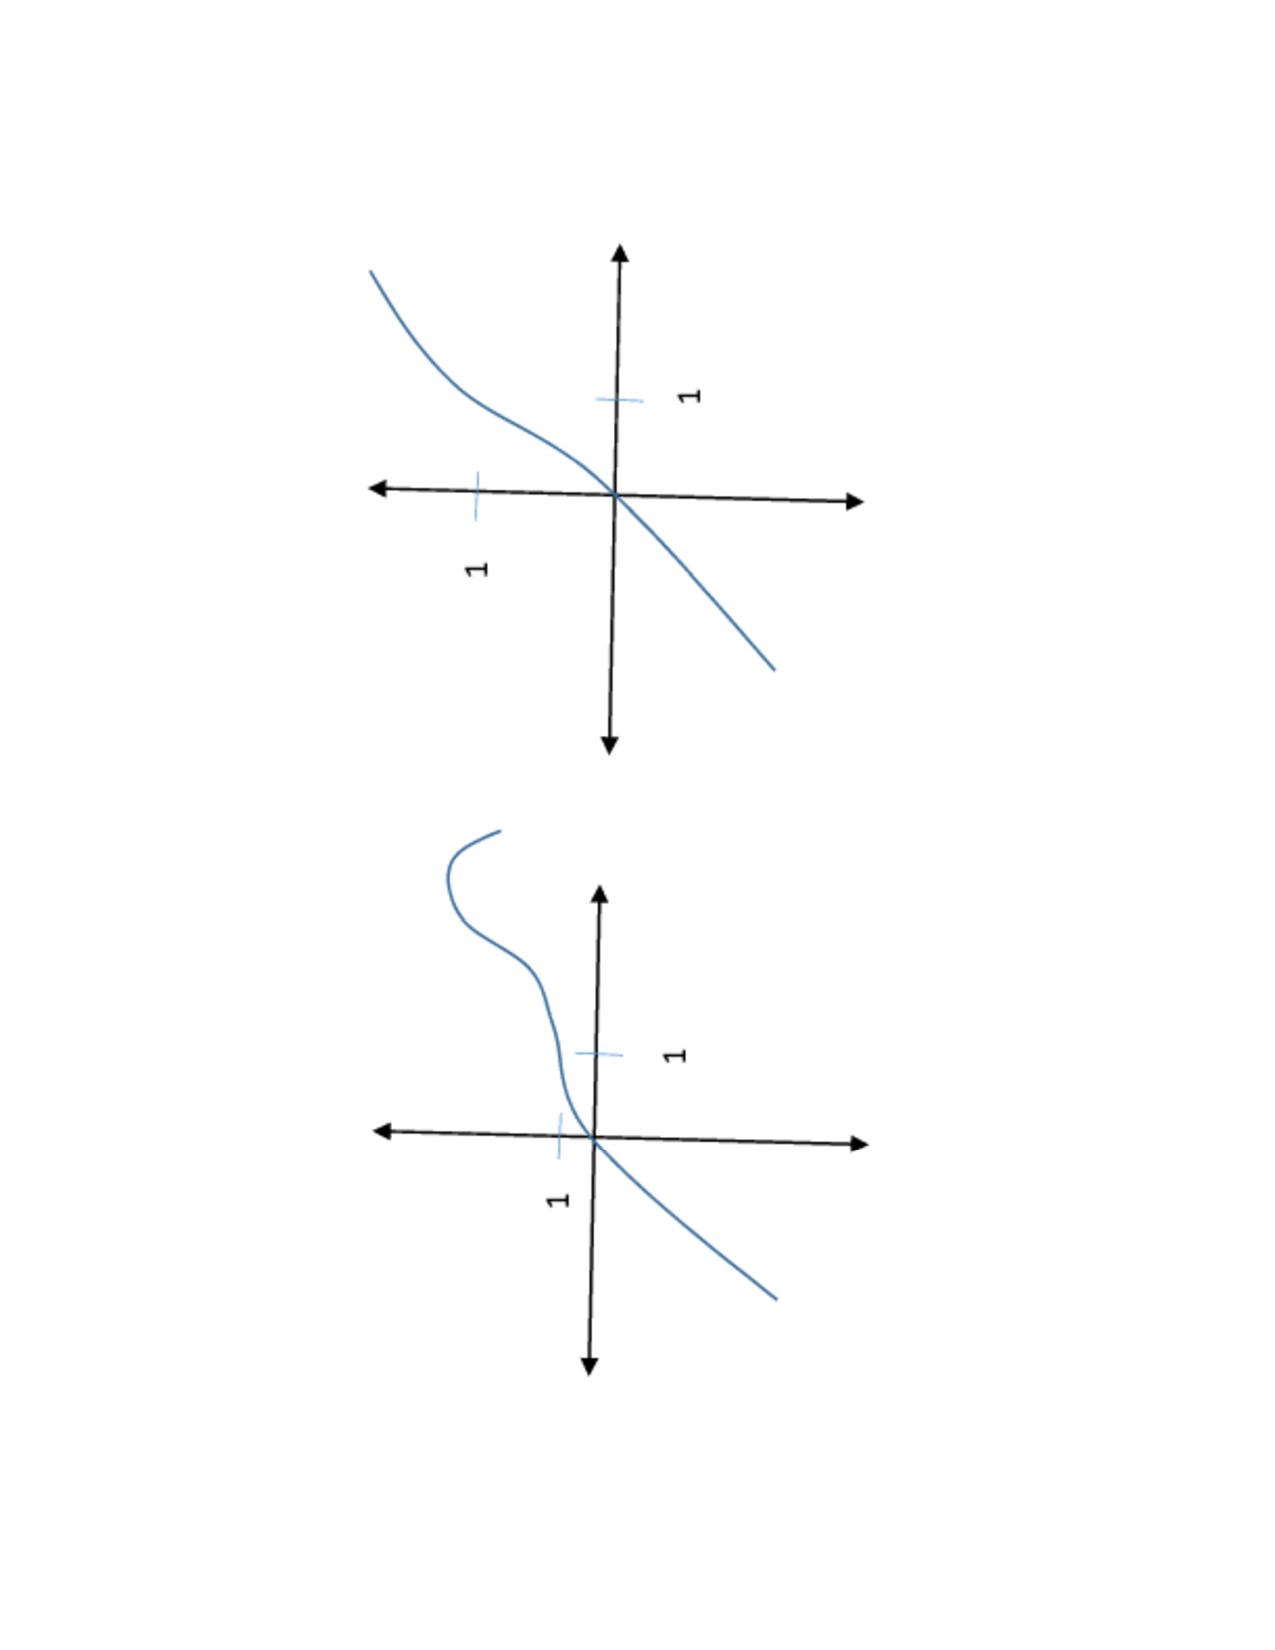
\includegraphics[trim= 170 200 190 180, scale=0.8, angle=-88.69]{Figure8-1-1.pdf}	
	\end{image}

	\begin{freeResponse}
	Since $y' = e^x (y-1)^2$, the derivative of $y$ is always nonnegative.  
	Thus, the first graph cannot satisfy this differential equation since it has a tangent line with a negative slope.
	
	\begin{image}
	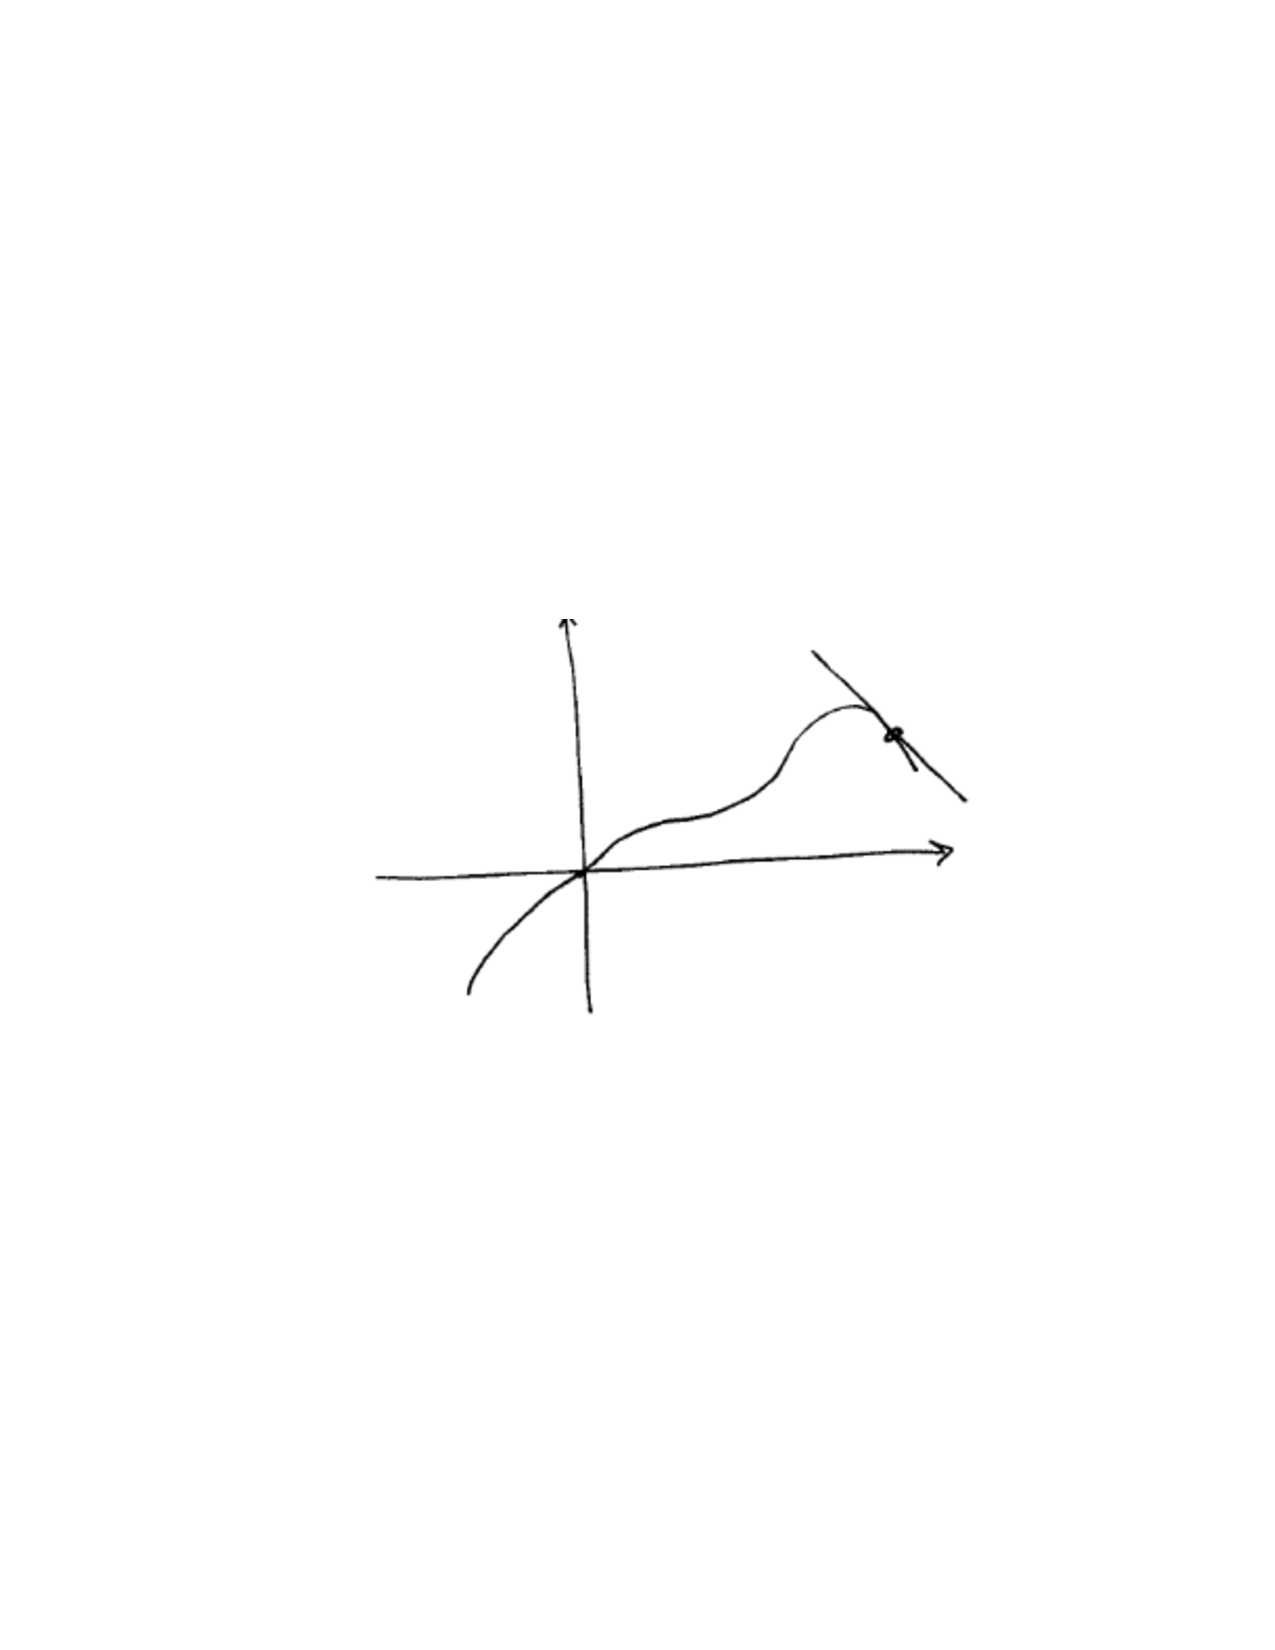
\includegraphics[trim= 170 300 190 310, scale=1]{Figure8-1-2.pdf}	
	\end{image}
	
	The second graph cannot satisfy the differential equation since the slope of the tangent line at $x=1$ is positive
	
	\begin{image}
	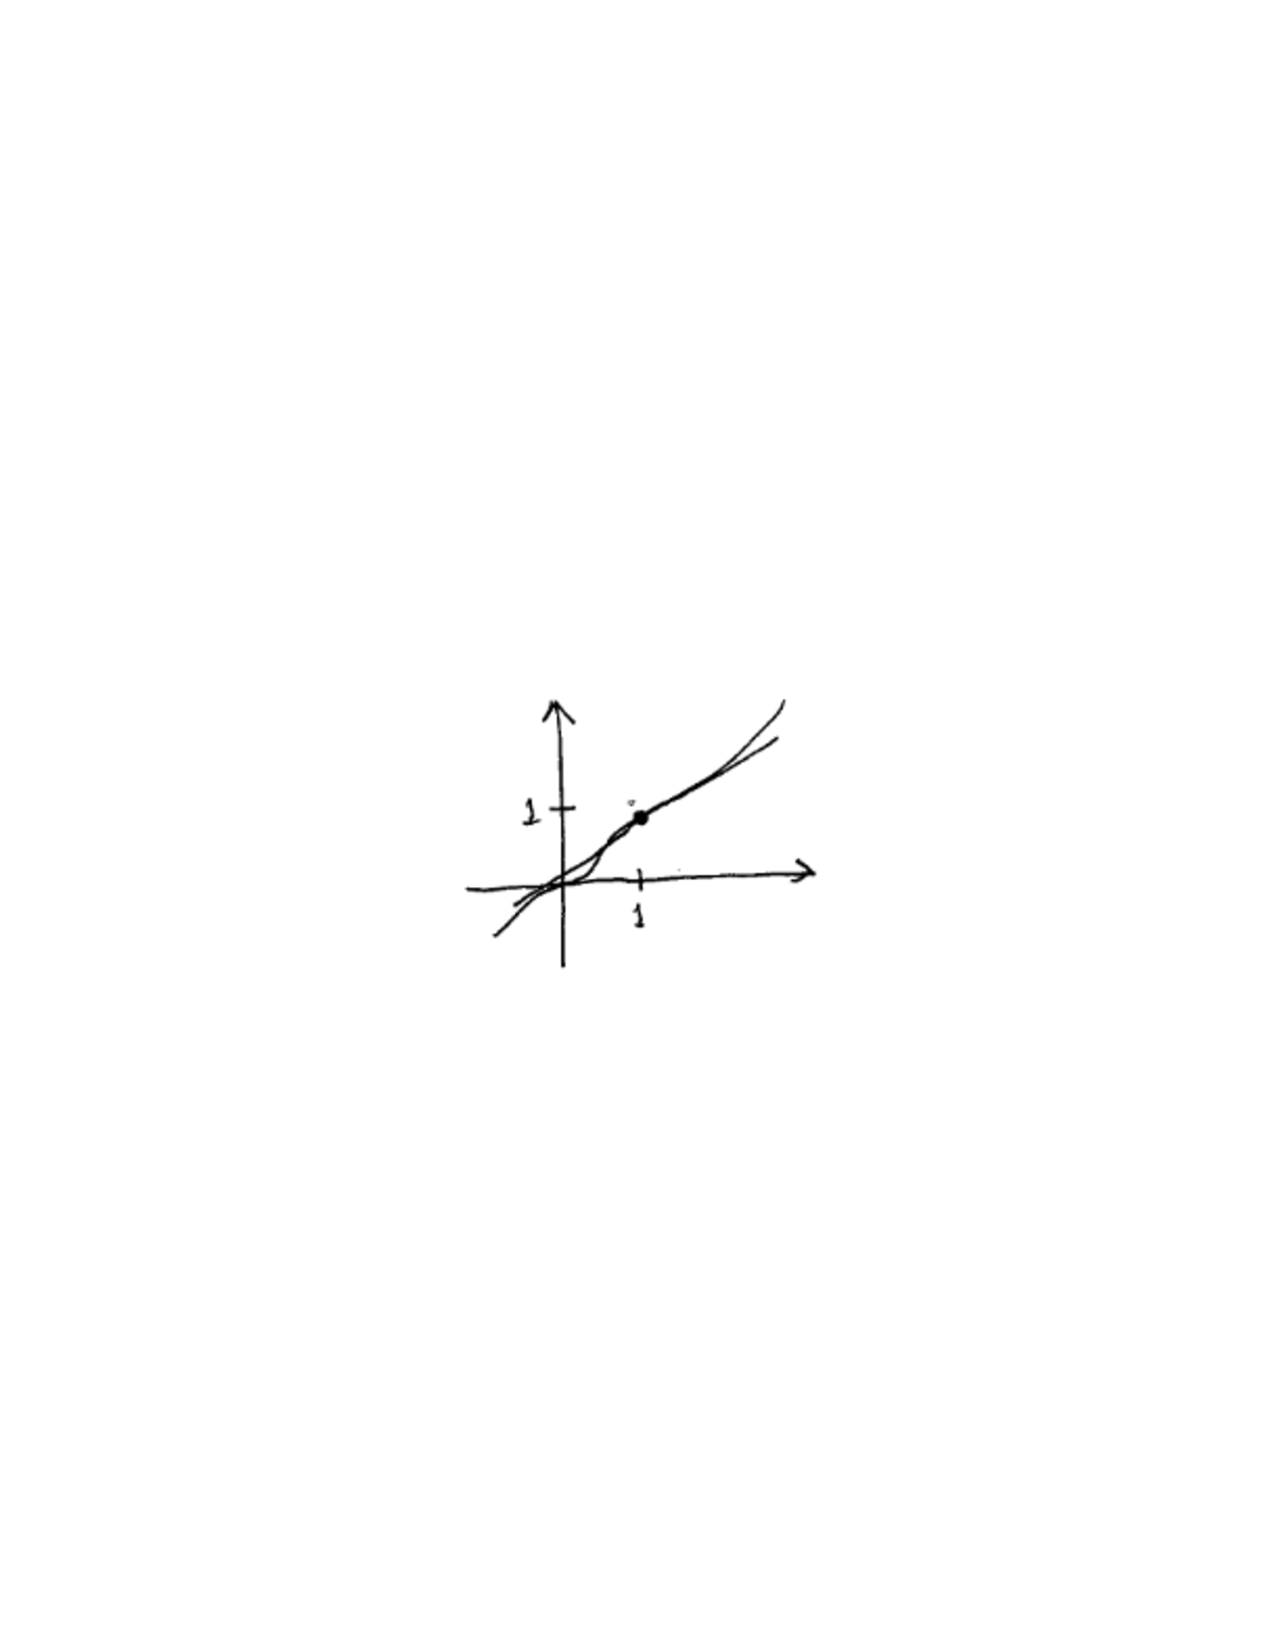
\includegraphics[trim= 170 330 190 330, scale=1]{Figure8-1-3.pdf}	
	\end{image}
	
	but $\eval{\dd[y]{x}}_{x=0} = e^0(1-1) = 0.$
	\end{freeResponse}

\end{problem}

\begin{instructorNotes}
This activity anticipates the idea of direction fields to be covered in Section 8.2.  
Students should eventually realize that differrential equations are statements about the slope of the function at each point $(x,y)$.  
Issues such as where the slope equals $0$ or where the slope is positive, negative, increasing, or decreasing should arise in the solution/discussion.  
The first graph has a negative slope at some places ($e^x$ and $(y-1)^2$ are always non-negative), and the second graph does not have a slope of $0$ at the point $(1,1)$.  
\end{instructorNotes}

\begin{instructorNotes}
This is a good exercise in evaluating differential equations with functions.  
Suggest that each member in the group try a different possible solution.
\end{instructorNotes}

\end{problem}














	
	
	
	
	
	
	
	
	

	










								
				
				
	







	
	
	
	
	
	
	
	
	

	










								
				
				
	














\end{document} 


















